\chapter{Time Series}

A \textbf{time series} is a collection of observations made sequentially in time, usually at constant time intervals. They can be constructed out of measurements of many different phenomenons, such as annual rainfall levels, earthquakes, fMRI data, quarterly earnings, audio/video data, and so on. Time series can analyzed through clustering, classification, motif discovery, rule discovery, forecasting, and trend/seasonality analysis. The key issues that arise when working with time series are:
\begin{itemize}
    \item \textbf{The amount of data to work with can be incredibly large}: for datasets with several different sources and short intervals of time between measurements, the size can be very high.

    \item \textbf{Similarity is not easy to estimate}: since series are complex objects with several values each, defining how two series can be considered similar is not as easy as it can be for numerical data.

    \item \textbf{Different data formats}: different series in the same dataset may be represented using a different scale or format; e.g., atmospheric temperatures recorded in both $^{\circ}C$ and $^{\circ}F$.

    \item \textbf{Different sampling rates}: while usually it is assumed that series are recorded all with the same rate, in many real life cases this may not be true. Different series may have different lengths and different time intervals.

    \item \textbf{Noise, missing values, and other defects}: as with other types of data, time series can also present noisy information or missing values.
\end{itemize}
The following sections will explain how some of these issues can be dealt with.

\section{Similarity Between Time Series}

\subsection{Structural-based Similarities}

Especially when analyzing long time series, similarity is calculated on a structural level. This means that global features are extracted from the time series, creating a feature vector, and measuring similarity looking at those features. Some examples are the mean and variance, maximum/minimum, skewness, mean and variance of the $1^{st}$ derivative, and so on.

A measure used to calculate structural dissimilarity is \textbf{compression based dissimilarity}, which is calculated as:
\begin{equation*}
    d(x,y) = \textit{CDM}(x,y) = \dfrac{C(x,y)}{C(x) + C(y)} \,,
\end{equation*}
where $C$ is a compression algorithm. The numerator is the compression of the concatenation of the two series, while the denominator is the sum of the compressions of the series done singularly: the Compression Dissimilarity Measure equal to 1 if the two series are unrelated, otherwise it is less than one. The smaller its value, the closer the series are to each other. CDM is never zero.

\subsection{Shape-based Similarities}

Shape-based similarities can be calculated using distance measures. Recall that distances have the following properties:
\begin{align*}
    &d(a,b) \geq 0, d(a,b) = 0 \iff a = b \ (\text{Positivity}) \\
    &d(a,b) = d(b,a) \ (\text{Symmetry}) \\
    &d(a,c) \leq d(a,b) + d(b,c) (\text{Triangle Inequality})
\end{align*}
One way to calculate shape-based dissimilarity is using Euclidean distance. Given two time series (with the same exact number of points/measurements), the Euclidean distance is calculated as if the series were points in an Euclidean space. However, this distance is very sensitive to distortions in the data, which should be removed in a preprocessing phase.\\
The most common distortions are:
\begin{itemize}
    \item \textbf{Offset translation}: the series have different offsets on the y axis. Calculating the distance without addressing this problem would return a value that is drastically larger than the actual shape distance. This can be corrected by subtracting each series with its own mean value.
    \begin{figure}[h]
        \centering
        \begin{minipage}{0.40\textwidth}
         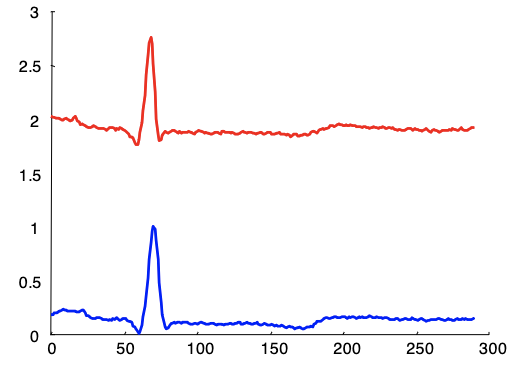
\includegraphics[width=1.0\linewidth]{img/offset_trans_1.png}
        \end{minipage}
        \hfill
        \begin{minipage}{0.40\textwidth}
            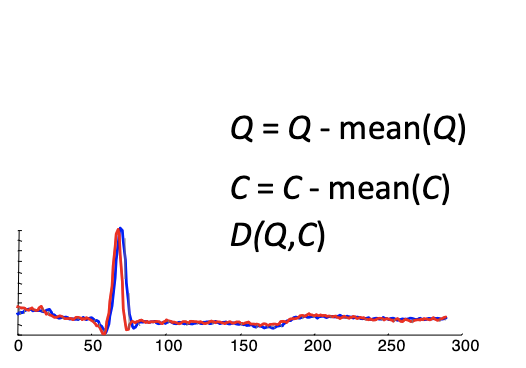
\includegraphics[width=1.0\linewidth]{img/offset_trans_2.png}
        \end{minipage}
        \label{fig:offset-trans}
        \caption{Offset translation transformation.}
    \end{figure}

    \item \textbf{Amplitude scaling}: the series have the same shape, but are scaled differently on the y axis. This is corrected by applying Z-score normalization to the values of the series (subtracting the mean and dividing by the standard deviation).
    \begin{figure}[h]
        \centering
        \begin{minipage}{0.40\textwidth}
            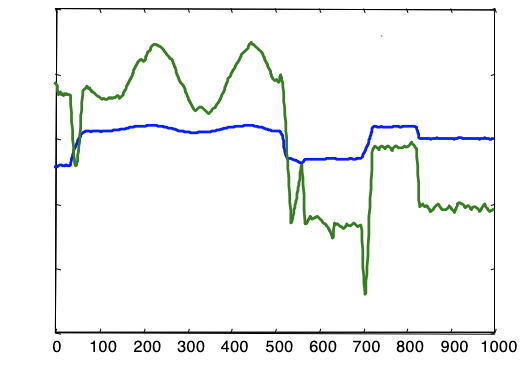
\includegraphics[width=1.0\linewidth]{img/ampli_scaling_1.png}
        \end{minipage}
        \hfill
        \begin{minipage}{0.40\textwidth}
            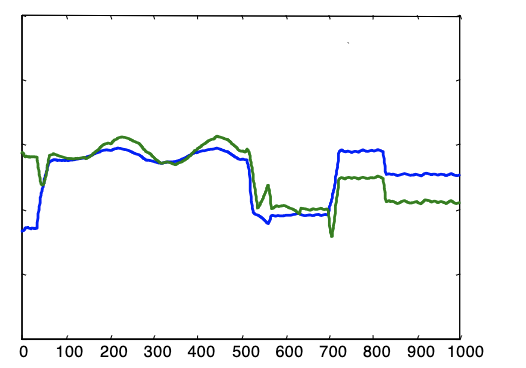
\includegraphics[width=1.0\linewidth]{img/ampli_scaling_2.png}
        \end{minipage}
        \caption{Amplitude scaling transformation.}
        \label{fig:ampli-scaling}
    \end{figure}

    \item \textbf{Linear trend}: series can follow upwards or downwards linear trends, which means that as they progress they increase or decrease in level. This can be corrected by finding the best fitting line to a time series, and subtracting it from the time series itself.
    \begin{figure}[h]
        \centering
        \begin{minipage}{0.40\textwidth}
            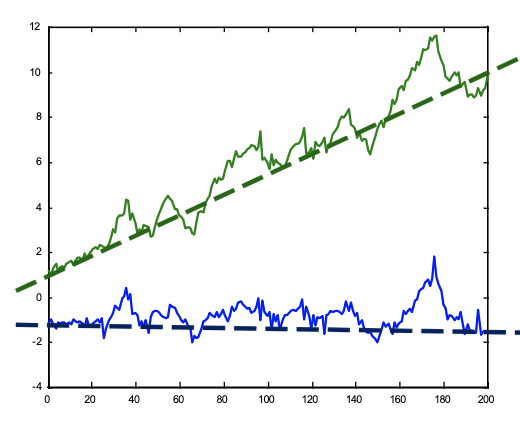
\includegraphics[width=1\linewidth]{img/lin_trend_1.png}
        \end{minipage}
        \hfill
        \begin{minipage}{0.40\textwidth}
            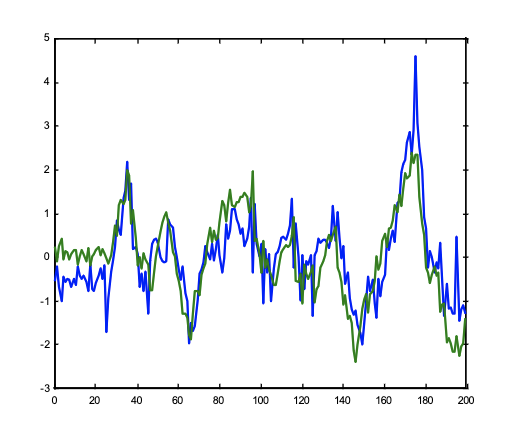
\includegraphics[width=1\linewidth]{img/lin_trend_2.png}
        \end{minipage}
        \caption{Linear trend transformation.}
        \label{fig:lin-trend}
    \end{figure}

    \item \textbf{Noise}: noise is the presence of random error in the series. To remove noise, each data point can be replaced with the average value of its neighbors.
    \begin{figure}[h]
        \centering
        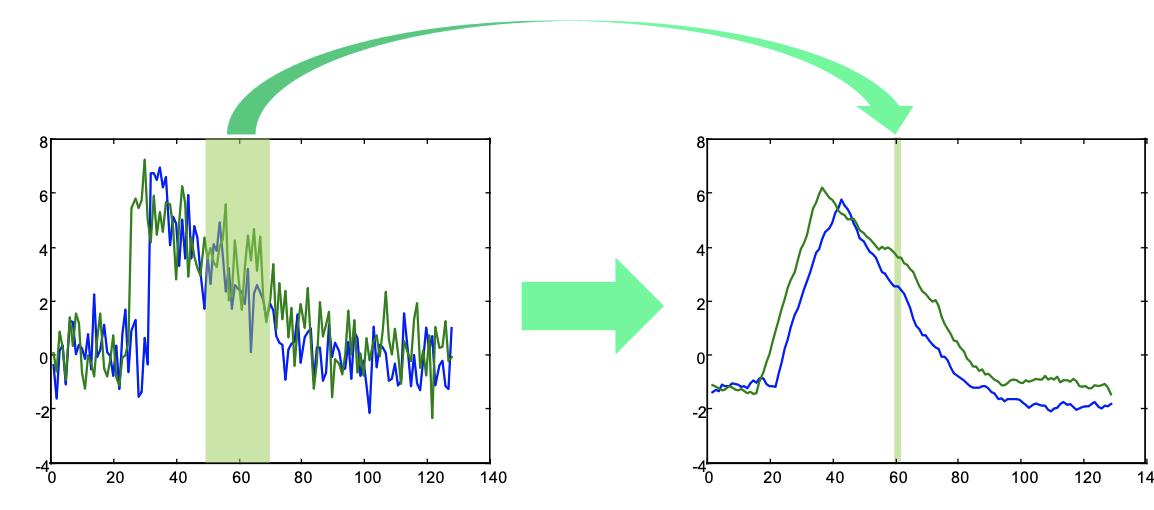
\includegraphics[width=0.9\linewidth]{img/noise_trans.png}
        \caption{Noise transformation.}
        \label{fig:noise-trans}
    \end{figure} \\
    Noise can be removed by a \textbf{moving average} (\textbf{MA}): given a window of length $w$ and a time series $t$, the MA is applied as:
    \begin{equation*}
        t_i = \dfrac{1}{w} \sum_{j=i-w/2}^{w/2} t_j \ i = 1, \dots , n
    \end{equation*}
\end{itemize}

\subsubsection{Dynamic Time Warping}

It's often the case that two time series have approximately the same shape, but they do not line up on the x axis. The euclidean distance calculated between such series would be high, despite them being similar: this is because it considers a fixed time axis for both series. In order to find the similarity between them, the time axis must be ``warped'' for one or both time series to align them correctly.

In practice, DTW is calculated in three steps. First, given the series $Q$ and $C$, a matrix of size $|Q| \times |C|$ is constructed, and each cell of index $i,j$ contains the distance between the $i^{th}$ component of $Q$ and the $j^{th}$ component of $C$. The diagonal of this matrix corresponds to the comparison done by the Euclidean distance. Every possible warping between two time series corresponds to a path from the bottom left corner $(0,0)$ and the top right corner $(0,|C|)$ of the matrix. The DTW will be the best path, i.e., the one that yields the lowest sum of costs. The best path is found recursively, using the following formula:
\begin{equation*}
    \gamma(i,j) = d(q_i,c_j) + \min\{\gamma(i-1, j-1), \gamma(i-1, j), \gamma(i, j-1)\}
\end{equation*}

The dynamic programming approach to the problem starts by calculating the distance matrix for the two series; then, the matrix of cumulative costs for each path; finally, the path with the best alignment is found, connecting the cells with the lowest cost.
\begin{figure}[h]
    \centering
    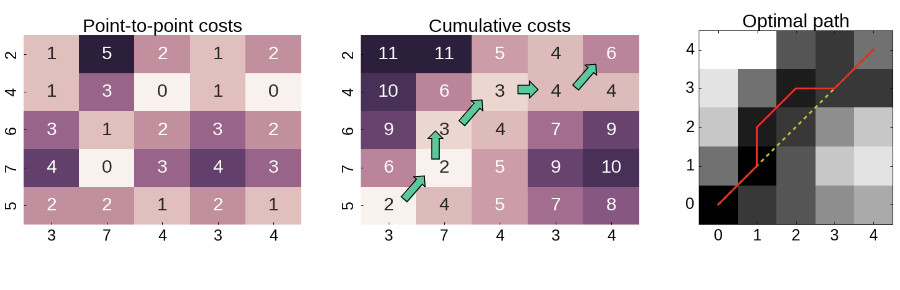
\includegraphics[width=1.0\linewidth]{img/dtw.png}
    \caption{How Dynamic Time Warping is calculated.}
    \label{fig:dtw}
\end{figure}

When the performances of Euclidean distance and DTW are compared for classification tasks, the former leads to much lower accuracy than the latter; however, DTW is also two to three orders of magnitude slower than Euclidean distance, meaning that it is unsuitable for larger datasets if used as is. In order to speed up the calculation of DTW, different approaches can be used depending on the length of the time series.

\begin{itemize}
    \item If the time series are short, then they can be \textbf{approximated} via compression or downsampling; alternatively, computation can be sped up by introducing \textbf{global constraints}.
    
    \item If the time series are long, compression/approximation-based dissimilarity can be used.
\end{itemize}

\paragraph{Global Constraints}

A global constraint limits the indices of the warping path $w_k = (i,j)_k$, such that $j-r \leq i \leq j+r$, where $r$ is an integer that defines the allowed range of warping for a given point in the series. This restricts the computation of distances and cumulative costs to a small window described by $r$. Two types of global constraints are the \textbf{Sakoe-Chiba Band} (restriction around the diagonal) and the \textbf{Itakura Parallelogram} (greater restriction at extremes of series, less restriction in the middle). Empirical analysis shows that given a dataset, the increase in the value of $r$ will rapidly improve performances, but after reaching a maximum they will decrease and then plateau.

\begin{figure}[h]
    \centering
    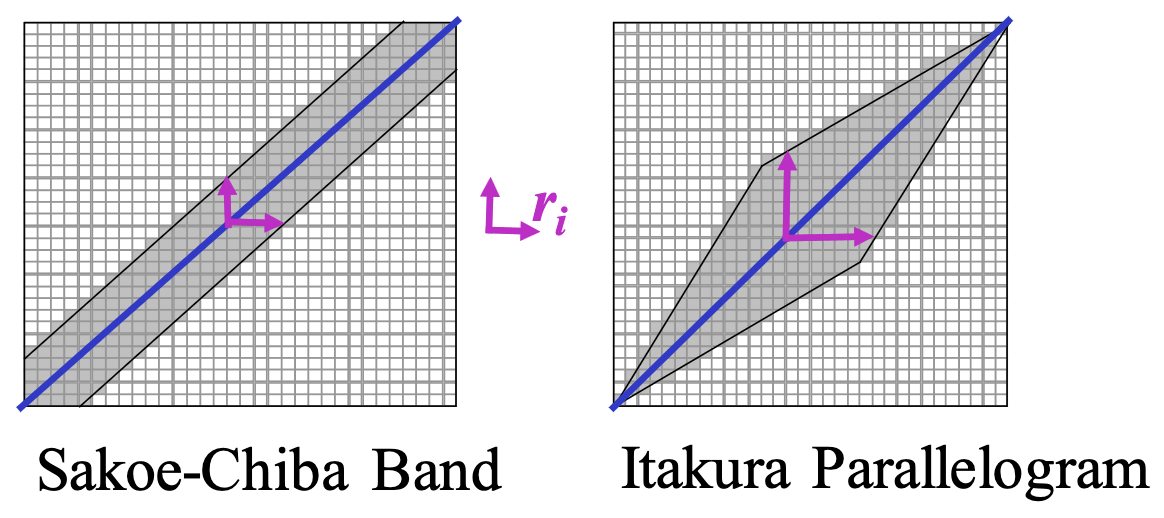
\includegraphics[width=0.7\linewidth]{img/dtw_global_constr.png}
    \caption{Global constraints.}
    \label{fig:dtw-global-constr}
\end{figure}

\paragraph{Approximation}

Approximation is a form of Dimensionality Reduction designed for time series. Compared to compression, approximation maps the series to a smaller space that is understandable, while the compressed space is not necessarily understandable.

\begin{itemize}
    \item \textbf{Discrete Fourier Transform (DFT)}: the time series is represented as a linear combination of sine and cosine functions, but only the first $n/2$ coefficients are kept. Each sine wave only requires 2 numbers: the phase and the amplitude. Many of the coefficients have very low amplitude, so they contribute very little to reconstructed signal: they can be discarded without significant loss of information, saving storage space.

    This approximation works great for most time series that represent natural signals, and many fast ($O(n \log(n))$) implementations exist. However, it struggles with series of different lengths and cannot support weighted distance measures. This approximation loses the temporal information of the original time series.

    \item \textbf{Discrete Wavelet Transform (DWT)}: the time series is represented as a linear combination of wavelet basis functions, but only the first $n$ coefficients are kept. Wavelets represent data in terms of sum and difference of a prototype wavelet, called analyzing/mother wavelet; they are localized in time, so some of the wavelet coefficients will represent small subsections of the data (unlike Fourier coefficients which always represent global contribution to data).

    This approximation has a good ability to compress stationary signals, and many fast ($O(n)$) implementations exist. However, it can only be defined for sequences whose length is an integral power of two; wavelets tend to approximate the left side of the sequence at the expense of the right one; it cannot support weighted distance measures. This approximation loses the temporal information of the original time series.

    \item \textbf{Singular Value Decomposition (SVD)}: the time series is represented as a linear combination of eigenwaves, but only the first $n$ coefficients are kept. This approach is similar to the previous two, but the eigenwaves are extracted from the data and are not a set of default waves.
    
    Time series can be thought of as points in a high-dimensional space, so the axes on which they are represented can be rotated so that axis 1 is aligned with the direction of maximum variance, axis 2 is aligned with the direction of maximum variance and is also orthogonal to axis 1, and so on, until the desired number of axes is obtained. Since the first eigenwaves will capture the most variance in the data, the rest can be truncated with little loss. This approximation loses the temporal information of the original time series.

    \item \textbf{Piecewise Linear Approximation (PLA)}: the time series is represented as a sequence of $k$ straight lines, which can be either connected or disconnected. Each line is described by its length and the height of its leftmost point; the height of the rightmost one can be inferred from the next segment.
    
    This approximation requires to choose the ``best'' value of $k$, that is, the optimal number of segments used to represent the time series that corresponds to the best trade-off between accuracy and compactness; this problem has no general solution.

    This approximation can efficiently compress data and filters noise. It also supports non-euclidean similarity measures.

    \item \textbf{Piecewise Aggregate Approximation (PAA)}: the time series is represented as a sequence of $N$ box basis functions, where each box has the same size. The mean value of the points in each segment is calculated, so that the approximation will be a series made up of several constant lines of fixed length. The dimensionality of the data is reduced from $n$ to $N$ (the number of segments). If $N=1$, the transformed representation is identical to the original series; if $N=n$, the approximation is a single segment equal to the mean of the entire series.

    This approximation is fast to calculate, supports Euclidean and non-Euclidean distance measures, as well as weighted Euclidean distance.
    
    \item \textbf{Adaptive Piecewise Constant Approximation (APCA)}: this approximation was developed as an extension of PAA. It allows the segments in the approximation to have different lengths, so that each segment is represented by two values: the first one corresponds to the mean value of the points falling within the same segment, the second one is its length.

    APCA can place bigger segments for areas of lower activity and many smaller segments for areas with higher activity (hence the ``adaptive''). In general, finding the optimal piecewise polynomial representation of a time series requires a $O(Nn^2)$ dynamic programming algorithm; in practice, however, an optimal representation is not needed, so fast algorithms ($O(n \log(n))$) to calculate high quality approximations exist. It supports Euclidean and non-Euclidean distance measures, as well as weighted Euclidean distance.

    \item \textbf{Symbolic Aggregate Approximation (SAX)}: a time series can be \textbf{segmented} using a predefined length $w$, predefined number of segments $k$, or using change point detection methods. SAX converts a time series into a discrete sequence of symbols, using a small alphabet size. Every part of the representation contributes about the same amount of information about the shape of the time series. The series is first normalized, and then two steps of discretization are performed.

    First, the time series of length $n$ is split into $w$ equal-sized segments, and each segment is approximated by the mean of all the points falling in it. Aggregating the resulting $w$ coefficients forms the PAA representation of the time series. Next, the breakpoints that divide the representation into $\alpha$ equiprobable regions are found, where $\alpha$ is the alphabet size (can be set by the user or derived from the Minimum Description Length). These breakpoints are chosen so that the probability of a segment falling into any of the regions is approximately the same: if the symbols were not equiprobable, some substrings would be more probable than others, introducing a probabilistic bias.

    Each region is assigned a different symbol from the chosen alphabet. The PAA coefficients can be mapped to the region to which they reside in a bottom-up fashion: the coefficients that fall in the lowest region are converted to $a$, the ones in the second lowest region to $b$, and so on. At the end, the representation will correspond to a sequence of symbols.
\end{itemize}
\clearpage
\begin{figure}[h]
    \centering
    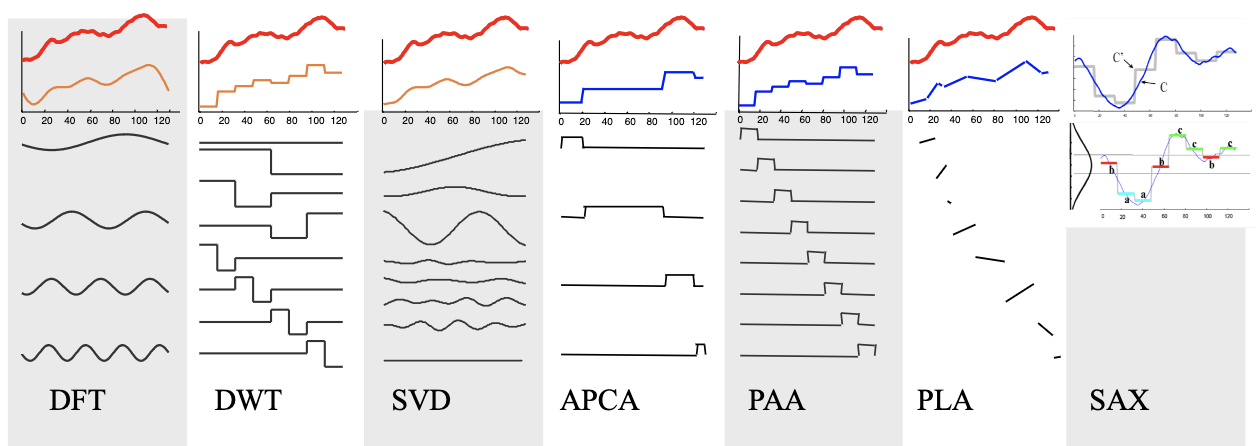
\includegraphics[width=1.0\linewidth]{img/approximations.png}
    \caption{The most common time series approximations.}
    \label{fig:approx-ts}
\end{figure}